\uuid{0LRR}
\exo7id{7136}
\auteur{megy}
\organisation{exo7}
\datecreate{2017-02-08}
\isIndication{true}
\isCorrection{true}
\chapitre{Géométrie affine euclidienne}
\sousChapitre{Géométrie affine euclidienne du plan}

\contenu{
\texte{
Soit $ABCD$ un quadrilatère convexe. On note $\mathcal B_A$ (resp. $\mathcal B_B$, $\mathcal B_C$, $\mathcal B_D$) la bissectrice intérieure en $A$ (resp. en $B$, $C$, $D$). Soient $I=\mathcal B_A\cap \mathcal B_B$, $J=\mathcal B_B\cap \mathcal B_C$, $K=\mathcal B_C\cap \mathcal B_D$ et $L=\mathcal B_D\cap \mathcal B_A$. Montrer que $IJKL$ est inscriptible.

\begin{center}
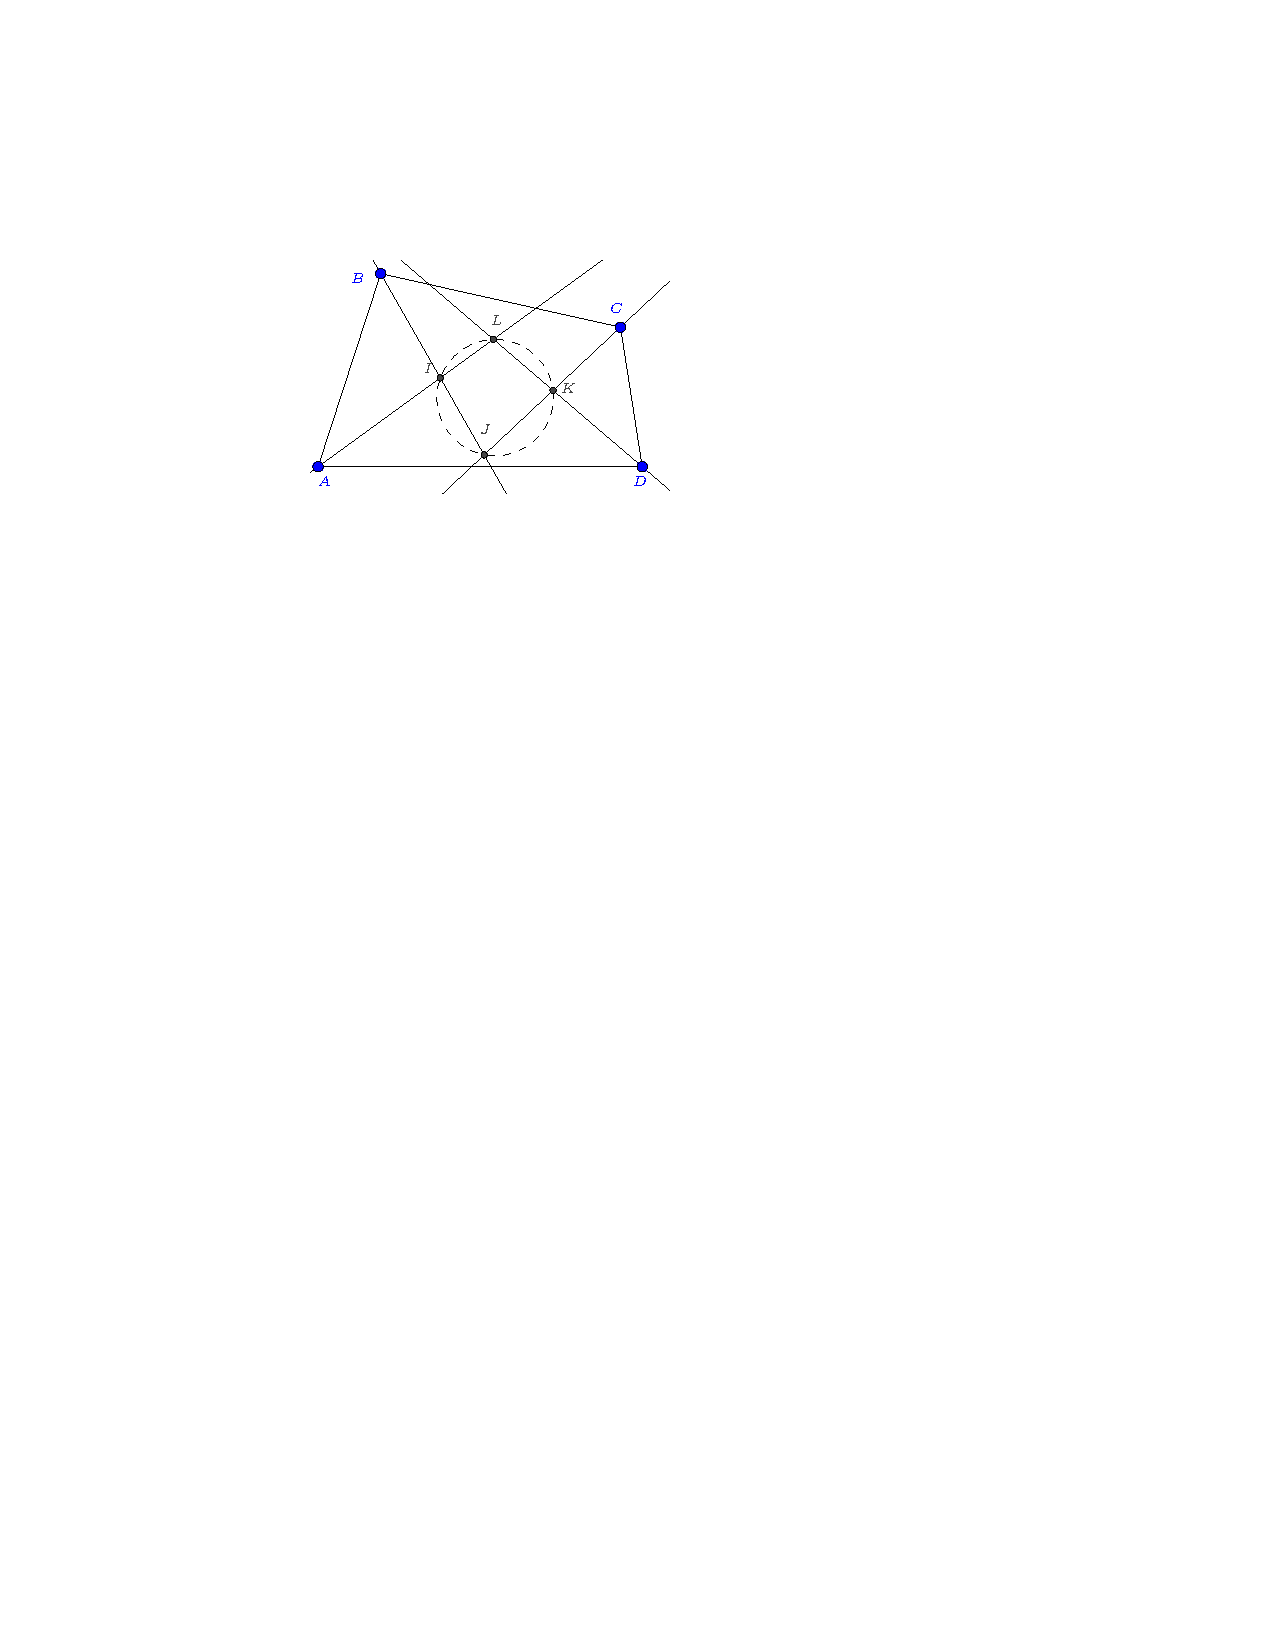
\includegraphics{../images/img007136-1}
\end{center}
}
\indication{La somme des angles d'un quadrilatère convexe vaut $2\pi$.}
\reponse{
La somme des angles d'un quadrilatère convexe vaut $2\pi$ :
\begin{align*}
2\pi &=
\widehat{ABC}+\widehat{BCD}+\widehat{CDA}+\widehat{DAB}\\
&= 2\widehat{ABI}
+2\widehat{KCD}+2\widehat{CDK}+2\widehat{IAB}
\end{align*}
d'où \[\widehat{ABI}
+\widehat{KCD}+\widehat{CDK}+\widehat{IAB}=\pi,\]
autrement dit la somme des demi-angles vaut $\pi$.

On termine alors la preuve en utilisant le critère de cocyclicité.
}
}
